\chapter{Preliminarii}

\section{Tipuri de învăţare automată}

Există numeroase tipuri de învăţare automată, aşa că le vom prezenta doar 
pe cele relevante lucrării noastre.

\subsection{Supervizată}

Învăţarea \textbf{supervizată} poartă acest nume deoarece necesită supraveghere 
umană pentru a putea funcţiona. Un specialist în ştiinţa datelor trebuie 
să parcurgă fiecare observaţie din setul de date şi să îi atribuie 
o \textbf{etichetă} corespunzătoare. Acest lucru este evident dificil, având în 
vedere că seturile de date cu minim sute de mii de entităţi sunt des întâlnite.

Această metodă este folosită în probleme de clasificare sau de prezicere 
a unor fenomene.

\subsection{Nesupervizată}

Învăţarea \textbf{nesupervizată} este opusul celei supervizate, deci implică faptul 
că interacţiunea umană nu este necesară în pregătirea setului de date. Cu toate 
acestea, rezultatele trebuie să fie interpretate de o persoană pentru a fi relevante,
întrucât nu mai avem etichete pe care să le folosim în evaluarea automată a 
performanţei.

Această metodă este folosită pentru a grupa datele în funcţie de similaritate,
a înţelege relaţia dintre punctele din setul de date şi pentru a face o analiză 
iniţială a datelor.

Toţi algoritmii din această lucrare aparţin acestei metode de învăţare automată.

\subsection{Semi-supervizată}

Învăţarea  \textbf{semi-supervizată} 
îmbină ambele paradigme prezentate anterior, astfel
că necesită un număr mic de date adnotate, lucru ce este evident mai uşor de 
obţinut faţă de un întreg set, şi un număr mare de date fara etichetă.

Această metodă este folosită spre exemplu în modelele ce se antrenează singure, 
folosind un algoritm supervizat antrenat pe datele adnotate ce este apoi 
folosit pe datele fara etichetă pentru a obţine un nou set de date adnotat.

Deşi această metodă nu este folosită în lucrarea noastră, am inclus-o deoarece 
ideea de bază în novelty detection cu metode nesupervizate este similară. Nu avem 
nevoie de date adnotate la antrenare şi este suficient un set mic pentru testarea 
ulterioară a performanţei.

\section{One Class SVM}

\subsection{Ideea algoritmului}

Această metodă este inspirată din clasificatorul cu vectori suport. Ideea este 
sa găsim \textbf{un hiperplan cu margine maximă}, posibil într-un spaţiu cu 
mai multe dimensiuni decât cel iniţial, în funcţie de kernel,
care să separe originea (se presupune că punctele sunt centrate) spaţiului de trăsături
de restul punctelor din setul de date\cite{scholkopf2000support}.

Un alt mod echivalent de a privi algoritmul este găsirea celei mai \textbf{mici 
hipersfere} care să includă toate punctele din setul de date\cite{tax2004support}.

\begin{figure}[H]
    \centering
    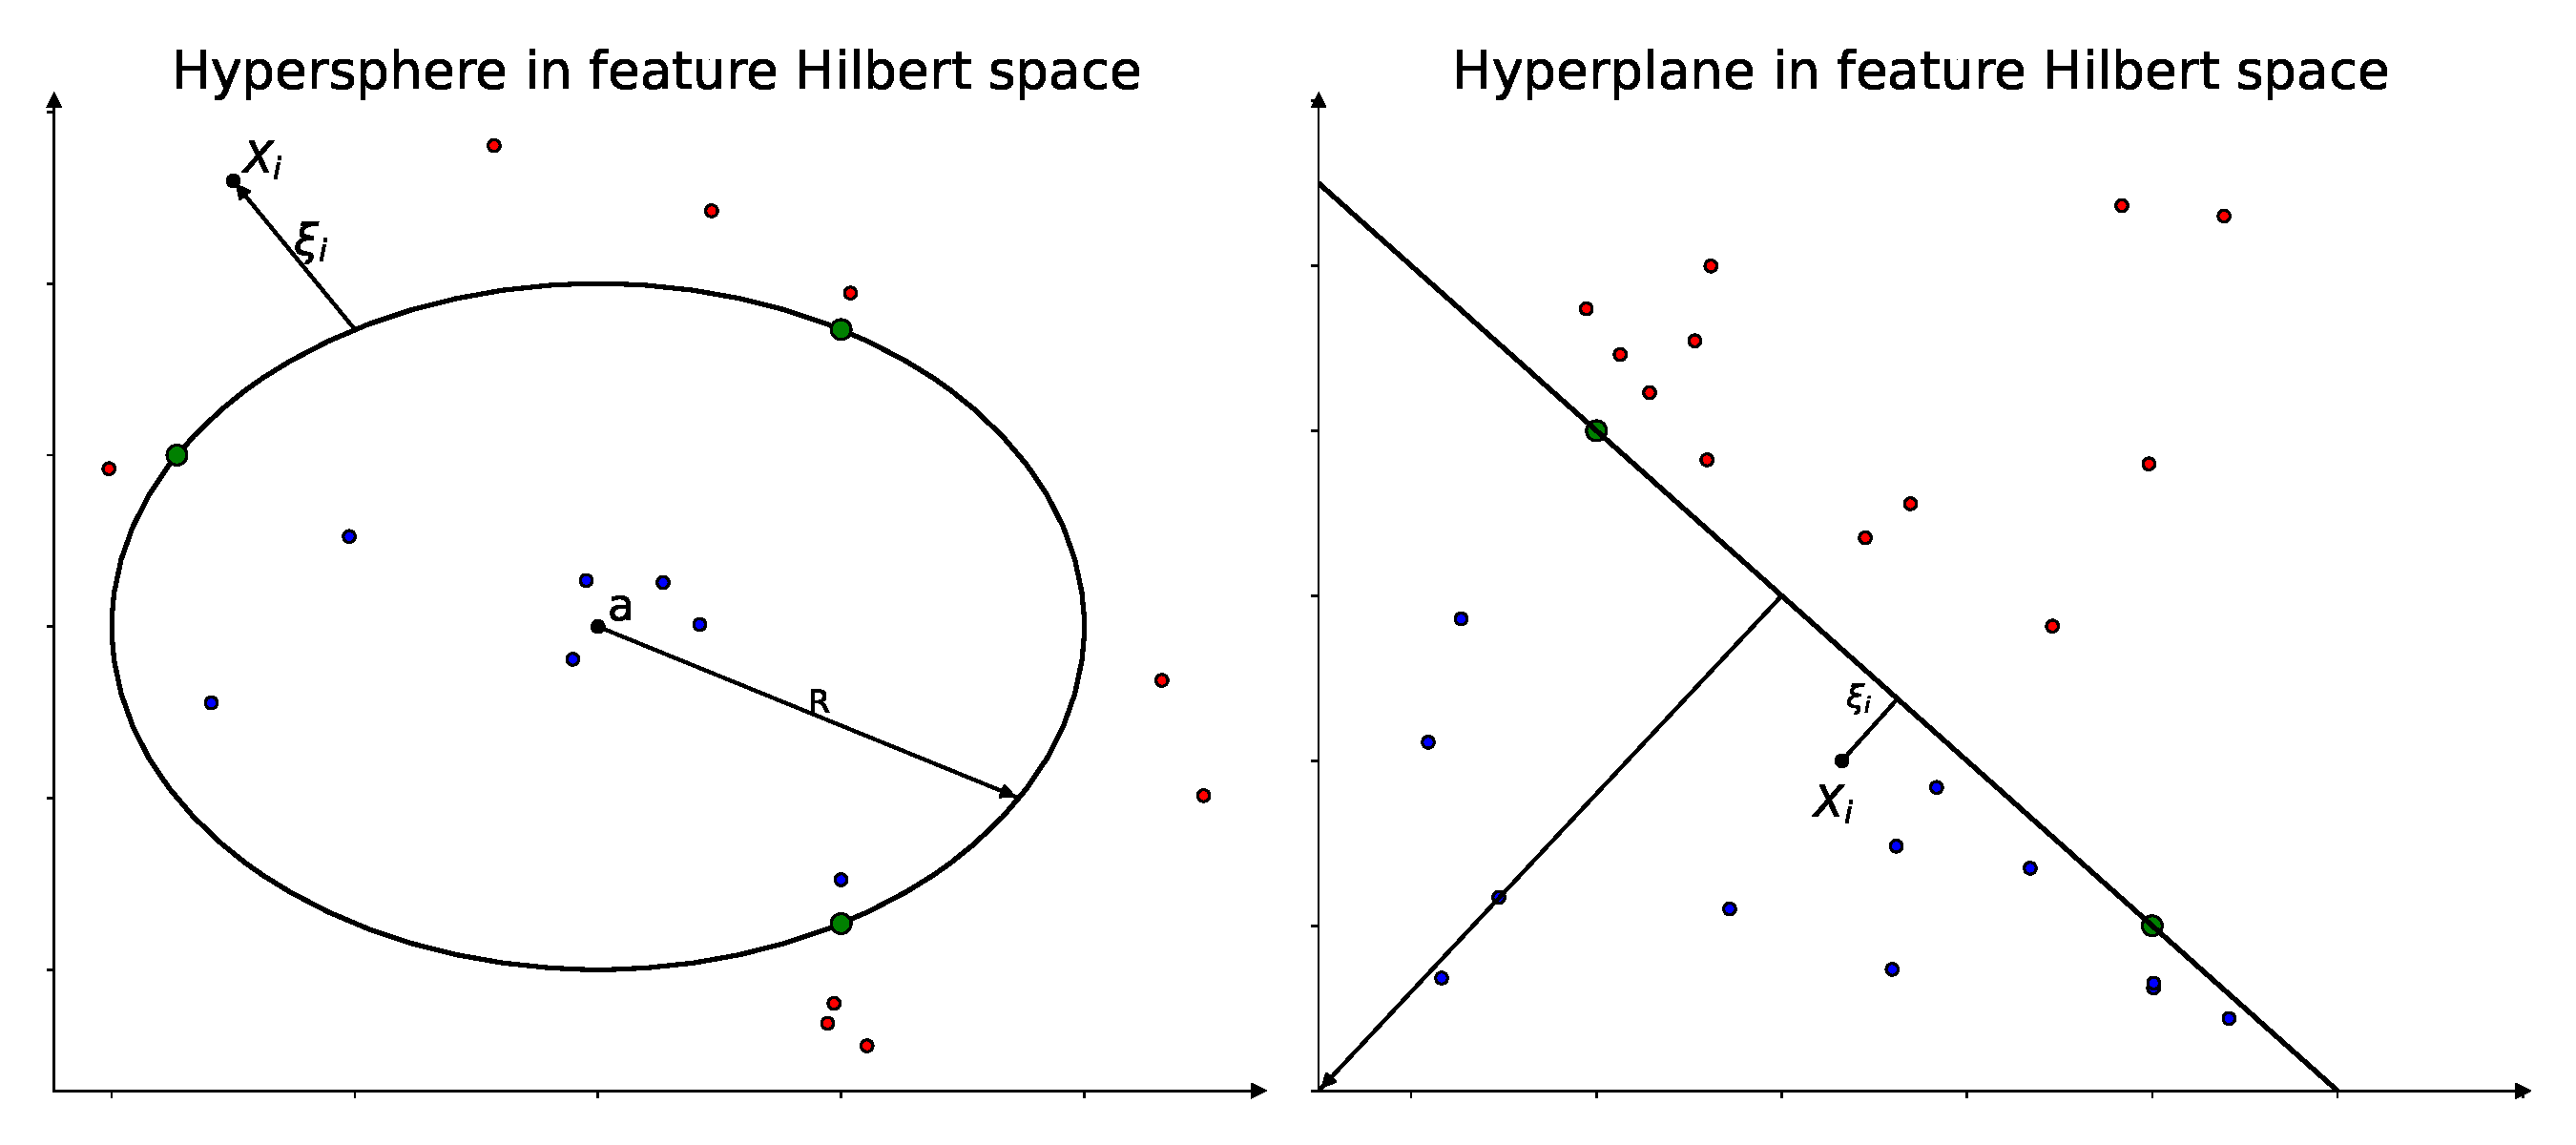
\includegraphics[width=\linewidth]{images/Hyperplane-Hypersphere.pdf}
    \caption{Varianta Schölkopf et al în dreapta şi varianta Tax et al în stânga}
\end{figure}

\subsection{Formularea matematică}

Prima formulare ce implică un hiperplan de separare

\begin{equation}
    \begin{aligned}
    & \underset{w, \rho, \xi}{\text{min}}
    & & \frac{1}{2} \|w\|^2 + \frac{1}{\nu n} \sum_{i=1}^{n} \xi_i - \rho \\
    & \text{cu constrângerea}
    & & \langle w, \phi(x_i) \rangle \geq \rho - \xi_i, \quad i=1,2,\ldots,n \\
    &&& \xi_i \geq 0, \quad i=1,2,\ldots,n \\
    \end{aligned}
    \end{equation}
    
    \begin{itemize}
        \item $w$ este vectorul de pondere al hiperplanului
        \item $\rho$ este termenul de influenţă
        \item $\xi_i$ sunt variabilele de relaxare pentru încălcarea marginii
        \item $\phi(x_i)$ este funcţia de scufundare pentru $x_i$.
        \item $n$ este numărul total de puncte
        \item $\nu$ este marginea superioară pentru ponderea de anomalii şi marginea 
        inferioară pentru ponderea de vectori suport
    
    \end{itemize}


    împreună cu forma sa duală ce implică folosirea unei funcţii kernel pentru găsirea unui hiperplan 
    de separare într-un spaţiu cu mai multe dimensiuni decât cel iniţial


    \begin{equation}
        \begin{aligned}
        & \underset{\alpha}{\text{min}}
        & & \frac{1}{2} \sum_{i=1}^{n} \sum_{j=1}^{n} \alpha_i \alpha_j K(x_i, x_j) \\
        & \text{cu constrângerea}
        & & 0 \leq \alpha_i \leq \frac{1}{\nu n}, \quad i=1,2,\ldots,n \\
        &&& \sum_{i=1}^{n} \alpha_i = 1
        \end{aligned}
        \end{equation}
    
    \begin{itemize}
        \item $\alpha_i$ sunt variabilele duale asociate punctelor 
        \item $K(x_i, x_j)$ este funcţia kernel
    \end{itemize}

A doua formulare ce implică găsirea hipersferei minime

    \begin{equation}
        \begin{aligned}
        & \underset{R, \rho, \xi}{\text{min}}
        & & R^2 + \frac{1}{\nu n} \sum_{i=1}^{n} \xi_i \\
        & \text{cu constrângerea}
        & & \|\phi(x_i) - c\|^2 \leq R^2 + \xi_i, \quad i=1,2,\ldots,n \\
        &&& \xi_i \geq 0, \quad i=1,2,\ldots,n \\
        \end{aligned}
        \end{equation}
        
        \begin{itemize}
        \item $R$ este raza hipersferei
        \item $c$ este centrul hipersferei
        \end{itemize}
        

\section{Gaussian Mixture Model}

\subsection{Ideea algoritmului}

Algoritmul încearcă să estimeze funcţia densitate de probabilitate 
din care au fost generate datele folosind 
\textbf{mai multe distribuţii Gaussiene}.
Astfel, putem modela distribuţii multimodale utilizând o distribuţie bine cunoscută.
Parametrii necesari sunt mediile şi covarianţele fiecărei componente.

\begin{figure}[H]
    \centering
    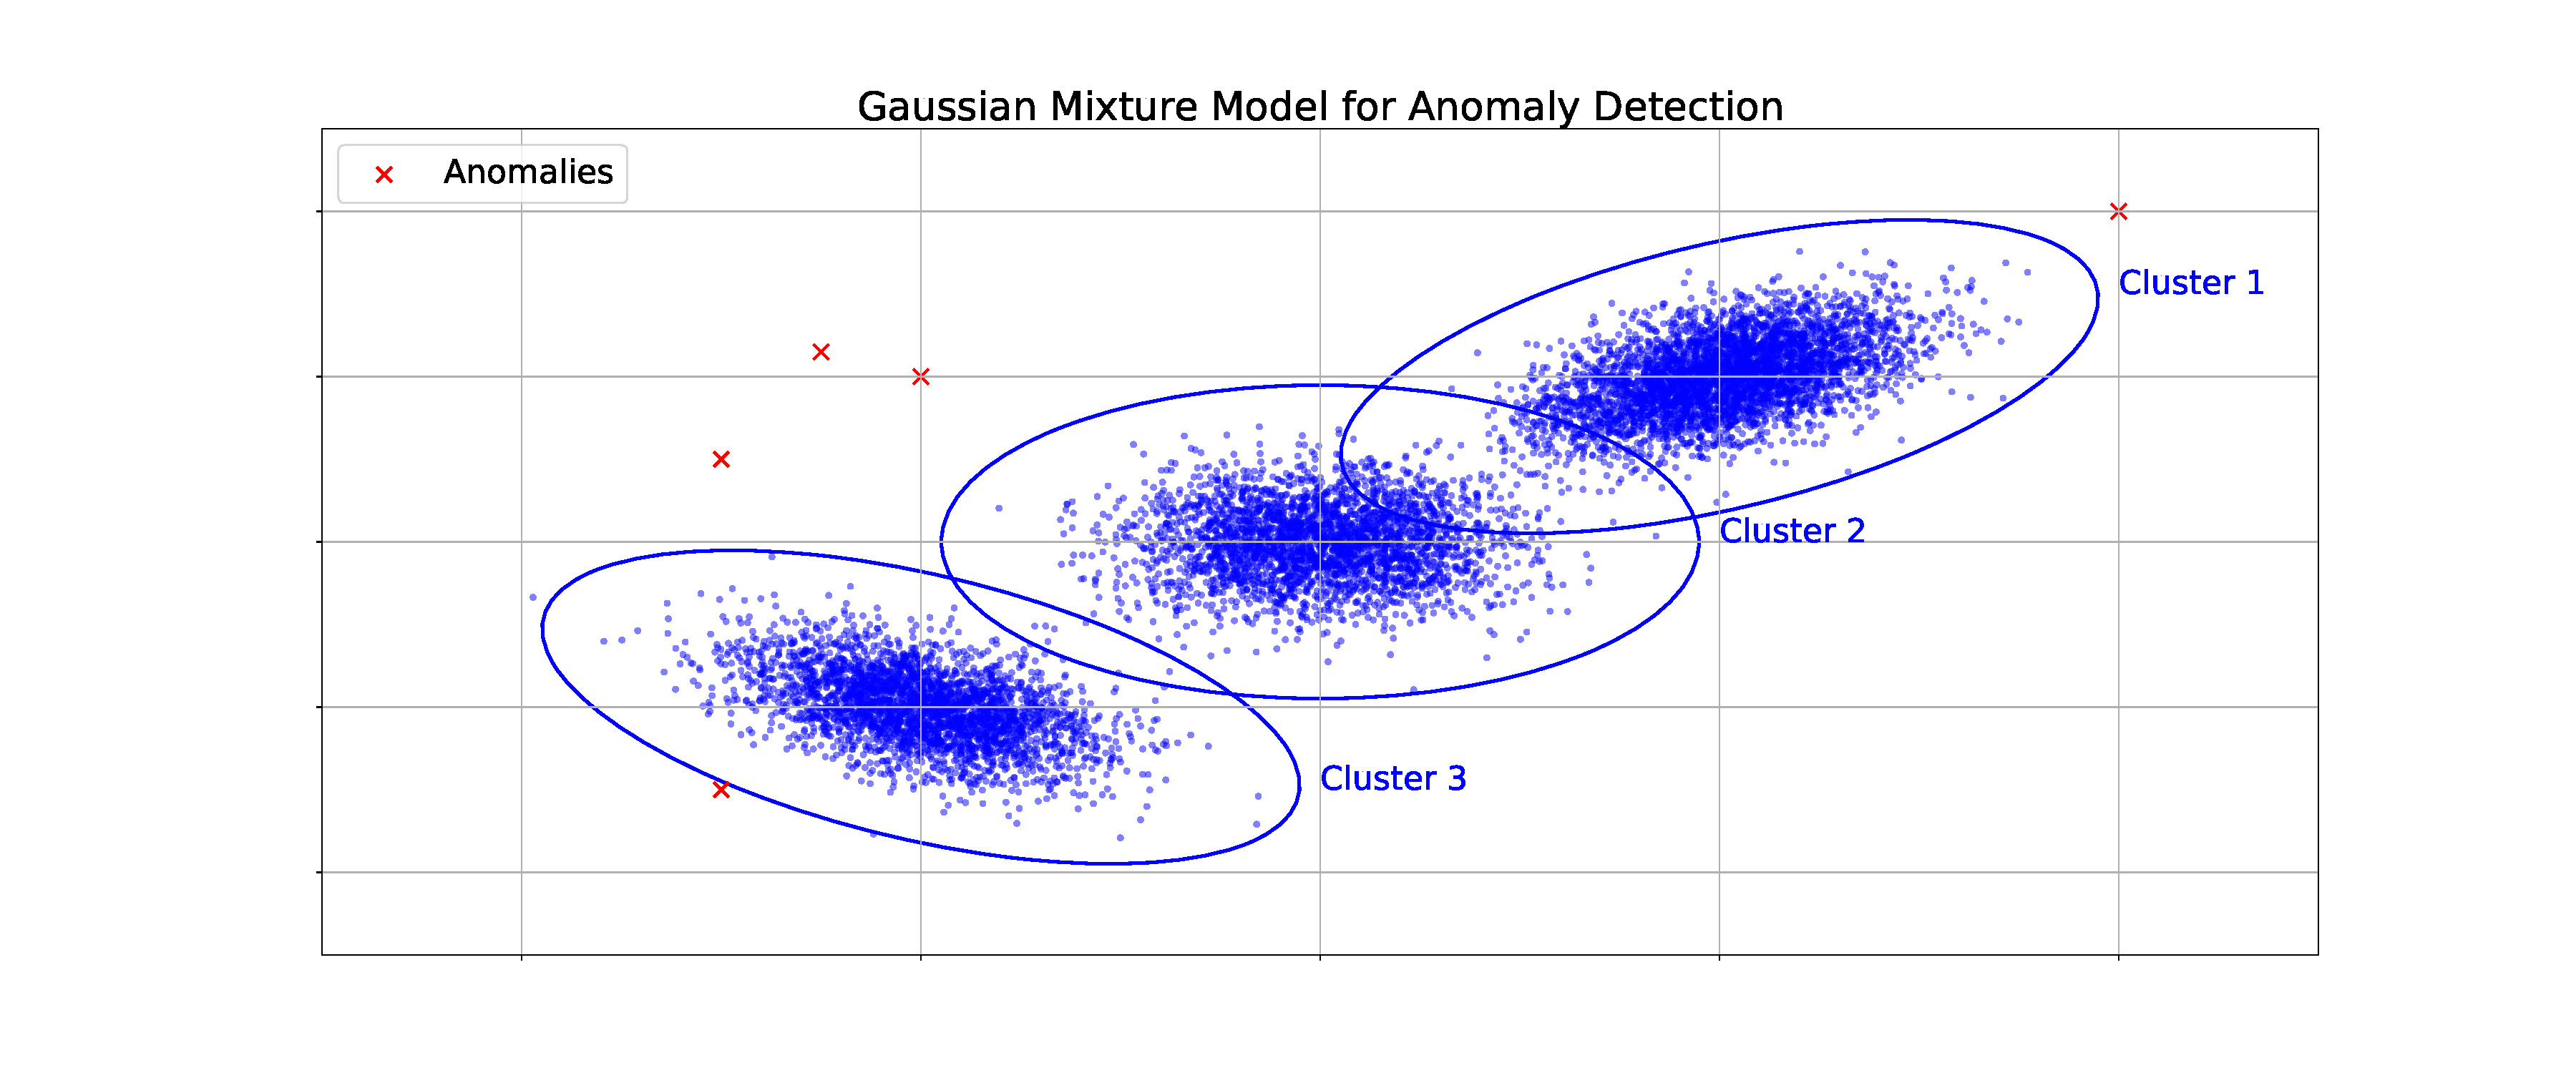
\includegraphics[width=\linewidth]{images/Anomaly-detection-with-Gaussian-mixture-models.pdf}
    \caption{Anomaliile se află în afara distribuţiilor date de componentele Gaussiene}
\end{figure}


\subsection{Formularea matematică}

Funcţia densitate de probabilitate estimată este dată de 

\begin{equation}
    \text{p}(x) = 1 - \prod_{i=1}^{K} \left(1 - \mathcal{N}(x|\mu_i, \Sigma_i)\right)
\end{equation}
    
\begin{itemize}
    \item $K$ este numărul de componente Gaussiene
    \item $\mathcal{N}(x | \mu_i, \Sigma_i)$ este distribuţia Gaussiană
    cu medie $\mu_i$ şi matrice de covarianţă $\Sigma_i$

Parametrii $\theta$ sunt de obicei învăţaţi din setul de date folosind 
tehnici precum algoritmul Expectation-Maximization (EM).
\end{itemize}

Această formulă ne indică probabilitatea ca un punct să fi fost generat de oricare 
dintre componentele Gaussiene implicate. Deci, o valoare cât mai mică sugerează 
o şansă mare ca punctul să fie anomalie.

\section{Kernel Density Estimation}

\subsection{Ideea algoritmului}

Precum Gaussian Mixture Model, algoritmul încearcă să estimeze 
funcţia densitate de probabilitate din care au fost generate datele.

Un parametru numit \textbf{"lăţime de bandă"} influenţează netezimea distribuţiei 
rezultate.
Cel mai des utilizat kernel este cel Gaussian şi pe acesta îl vom folosi şi noi.

Aici, pentru fiecare punct generăm o distribuţie Gaussiană cu \textbf{media} egală
cu punctul respectiv şi \textbf{deviaţie} egală cu "lăţimea de bandă". Apoi, adunăm toate 
distribuţiile obţinute mai sus si le împărţim la numărul total de puncte.

\begin{figure}[H]
    \centering
    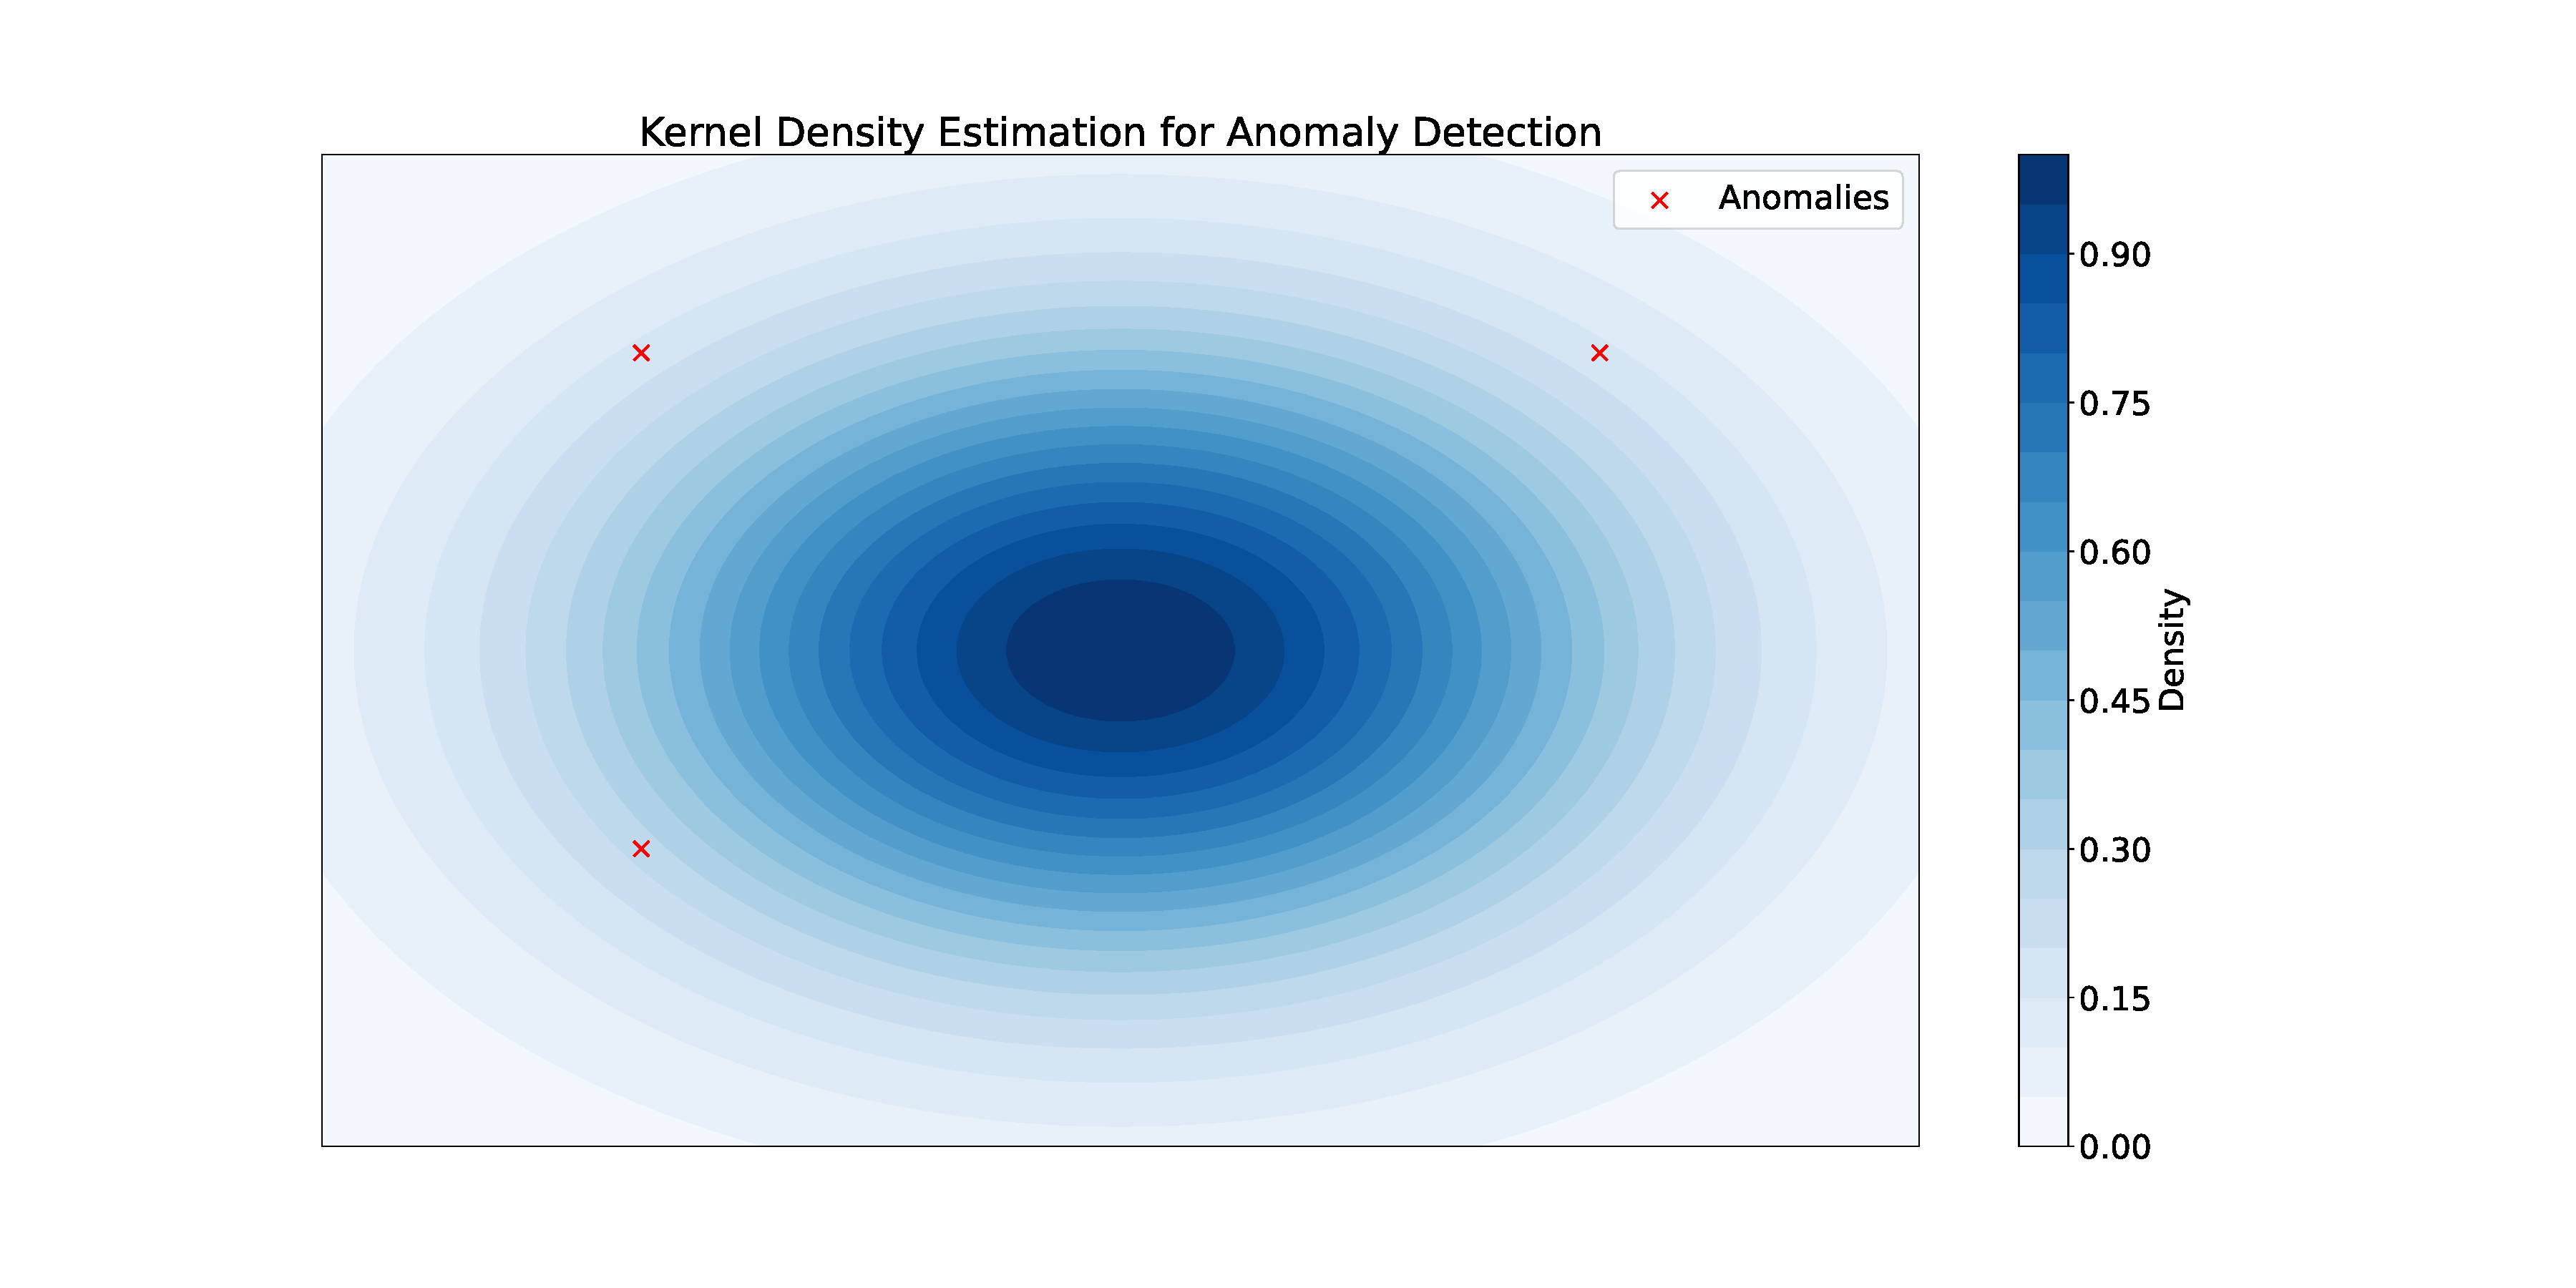
\includegraphics[width=\linewidth]{images/KDEShowOff.pdf}
    \caption{Anomaliile sunt reprezentate de punctele roşii}
\end{figure}

\subsection{Formularea matematică}

Densitatea estimată de kernel într-un punct $x$ este dată de

\begin{equation}
\hat{f}_h(x) = \frac{1}{nh} \sum_{i=1}^{n} K\left(\frac{x - x_i}{h}\right)
\end{equation}

\begin{itemize}
    \item $n$ este numărul total de puncte
    \item $h$ este lăţimea de bandă
    \item $K(u)$ este funcţia kernel 
\end{itemize}

\section{Metrici de performanţă}

Setul de date prezentat în această lucrare este adnotat în întregime, aşa 
că putem folosi aceleaşi tehnici de evaluare a performanţei utilizate pentru
clasificarea binară.

Prin urmare, are sens să folosim următoarele noţiuni ce vor fi utile pentru
descrierea metricilor de performanţă prezentate mai jos:

\begin{itemize}
    \item \textbf{TP} (\textit{true positive}) - reprezintă observaţiile din clasa 
    \textbf{pozitivă} ce au fost clasificate \textbf{corect}
    \item \textbf{TN} (\textit{true negative}) - reprezintă observaţiile din clasa 
    \textbf{negativă} ce au fost clasificate \textbf{corect}
    \item \textbf{FP} (\textit{false positive}) - reprezintă observaţiile din clasa 
    \textbf{pozitivă} ce au fost clasificate \textbf{greşit}
    \item \textbf{FN} (\textit{false negative}) - reprezintă observaţiile din clasa 
    \textbf{negativă} ce au fost clasificate \textbf{greşit}
\end{itemize}
În cazul nostru, clasa \textbf{pozitivă} este reprezentată de \textbf{anomalii}, iar 
clasa \textbf{negativă} este reprezentată de datele \textbf{normale}.

Metricile descrise în această lucrare reprezintă o alegere personală pe care o facem, astfel
încât să reflecte cât mai bine nevoile problemei expuse şi nicidecum nu reprezintă singura
sau cea mai bună cale de a evalua performanţa algoritmilor. Putem pune în paralelă cu teorema
\textbf{"No Free Lunch"} care ne spune că nu există un model care să fie cel mai bun în toate situaţiile,
ci că utilitatea acestuia depinde strict de context. La fel este şi în cazul măsurilor de evaluare,
iar acest fapt face găsirea uneltei potrivite pentru problemă una nu tocmai simplă, ba chiar 
poate necesita un timp considerabil de gândire.

\subsection{Accuracy}

\begin{equation}
    \text{Accuracy} = \frac{TP + TN}{TP + TN + FP + FN}
\end{equation}

Această metrică ne indică câte 
\textbf{clasificări făcute de model au fost corecte din 
totalul de puncte care trebuie clasificate}.

\subsection{Precision}

\begin{equation}
    \text{Precision} = \frac{TP}{TP + FP}
\end{equation}

Precision ne indică \textbf{capacitatea modelului de a nu produce fals pozitive}, în cazul nostru,
de a nu raporta o valoare normală ca fiind anomalie.

\subsection{Recall}

\begin{equation}
    \text{Recall} = \frac{TP}{TP + FN}
\end{equation}

Recall ne indică 
\textbf{capacitatea modelului de a identifica toate observaţiile pozitive},
în cazul nostru, de a detecta toate anomaliile.

\subsection{F1 score}

\begin{equation}
    \text{F1 Score} = \frac{2 \cdot \text{Precision} \cdot \text{Recall}}{\text{Precision} + \text{Recall}}
\end{equation}

F1 score reprezintă \textbf{media armonică dintre precision şi recall}. Prin urmare, f1 score 
va tinde către valoarea mai mică dintre aceste 2 metrici. Pentru a o maximiza,
ar trebui sa avem o valoare mare atât pentru precision, cât şi pentru recall,
fapt ce ar duce la un model ideal.

\subsection{AUC şi ROC Curve}

ROC Curve ne ajută să evaluăm calitatea modelului prin reprezentarea grafică 
a ratei de fals pozitiv pe axa X şi a ratei de adevărat pozitiv pe axa Y. 
\textbf{Punctul 
ideal al graficului se află în colţul din stânga sus} pentru ca ne dorim o 
rată de fals pozitiv egală cu 0 şi o rată de adevărat pozitiv egală cu 1. Prin urmare,
ne dorim sa maximizăm rata de adevărat pozitiv şi de a minimiza rata de fals pozitiv.

Pentru a crea graficul, avem nevoie de \textbf{probabilităţile sau valorile de încredere} 
pentru fiecare observaţie din setul de  testare, generate de funcţia de decizie a 
modelului respectiv. Punctele de pe grafic pot fi văzute precum clasificatoare 
separate ce diferă prin \textbf{pragul} aplicat funcţiei de decizie. Prin urmare, dacă
dorim să ilustrăm ROC Curve, avem nevoie de un algoritm ce are ca valori de ieşire
scoruri care pot fi comparate. One Class SVM, prin definiţie, nu oferă astfel de 
rezultate, aşa că va trebui să îl tratăm în mod diferit.

\textbf{Funcţia de decizie} este cea care atribuie un scor pentru 
un punct din set cu scopul de a indica nivelul de normalitate sau de anomalie 
al acestuia. Generarea etichetei se face apoi folosind un prag în cazul 
probabilităţilor, precum Gaussian Mixture Model şi Kernel Density Estimation, 
sau efectiv reducând valorile pozitive la $+1$ şi pe cele negative la $-1$,
precum One Class SVM.

Totuşi, ROC Curve are caracter vizual şi nu ne oferă o măsură concretă a performanţei.
De aceea, avem nevoie de \textbf{AUC}, valoare ce reprezintă aria de sub grafic. Cu cât aria
este mai mare, cu atât modelul este mai bun.

\subsection{Micro average vs Macro average}

Nu există o singură metodă de evaluare a modelelor care să fie potrivită în toate 
cazurile. În schimb, metodele sunt alese astfel încât să reflecte cât mai bine 
nevoile problemei.

\textbf{Macro} average pentru o măsură de evaluare are forma:

$$B_{macro}=\frac{1}{q} \sum_{\lambda=1}^{q} B(tp_{\lambda}, tn_{\lambda}, fp_{\lambda},
fn_{\lambda})$$

\textbf{Micro} average pentru o măsură de evaluare are forma:

$$B_{micro}=B(\sum_{\lambda=1}^{q} tp_{\lambda}, \sum_{\lambda=1}^{q} tn_{\lambda}, 
\sum_{\lambda=1}^{q} fp_{\lambda}, \sum_{\lambda=1}^{q} fn_{\lambda})$$

$L=\{\lambda_{j}: j=1,\dots,q \}$ este setul tuturor etichetelor asociate claselor, iar 
$B(tp, tn, fp, fn)$ este o măsură de evaluare binară bazată pe noţiunile introduse mai sus
\cite{Asch2013MacroandME}.
În cazul nostru, $\lambda=2$.


Diferenţa între cele 2 metode este că macro average acordă o importanţă 
\textbf{egală fiecărei 
clase}, pe când micro average acordă o importanţă 
\textbf{egală fiecărei observaţii}. Prin urmare,
varianta micro favorizează clasa 
\textbf{majoritară} la calcularea scorului, în timp ce varianta 
macro favorizează clasa \textbf{minoritară}.

Ilustrăm aceste diferenţe printr-un exemplu ce are ca măsură de evaluare binară 
\textbf{accuracy},
şi care arată cum metodele acoperă nevoi diferite.

Ponderea claselor este extrem de neechilibrată în setul nostru de date, anomaliile 
reprezentând doar $0.017\%$ din total. Prin urmare, dacă dorim să maximizăm 
micro average accuracy, putem alege un model trivial ce mereu prezice clasa majoritară.
Am obţine un accuracy de peste $99.9\%$ cu un minim de efort!

Este impresionant, dar modelul de mai sus este practic inutil pentru problema noastră.
Toate anomaliile ar trece nedetectate. În schimb, dacă am evalua acelaşi model folosind
varianta macro average, am obţine un accuracy de doar $50\%$. Modelul este acum inutil,
întrucât suntem interesaţi să detectăm anomaliile, nu doar să punem eticheta corectă 
pe cât mai multe observaţii indiferent de clasă.

Astfel, vom folosi varianta macro average pentru accuracy, iar pentru precision, recall şi 
f1 score, vom calcula rezultatul folosind clasa minoritară ca referinţă. Decizia este influenţată
de faptul că vrem să urmărim performanţa modelului pe detectarea anomaliilor în special, cu ajutorul
precision şi recall, dar în acelaşi timp vrem să obţinem un echilibru între fals pozitive şi 
adevărat pozitive, utilizând accuracy împreună cu f1 score, metode ce iau în calcul performanţa 
per total pe ambele clase. Este important să detectăm cât mai multe fraude, dar în acelaşi timp 
nu ne dorim să semnalăm un număr prea mare de tranzacţii ca fiind problematice deoarece modelul 
ar deveni un inconvenient.